\documentclass[a4paper,14pt, unknownkeysallowed]{extreport}

\usepackage{cmap} % Улучшенный поиск русских слов в полученном pdf-файле
\usepackage[T2A]{fontenc} % Поддержка русских букв
\usepackage[utf8]{inputenc} % Кодировка utf8
\usepackage[english,russian]{babel} % Языки: русский, английский
\usepackage{enumitem}

 
\usepackage{threeparttable}

\usepackage[14pt]{extsizes}

\usepackage{caption}
\captionsetup{labelsep=endash}
\captionsetup[figure]{name={Рисунок}}

% \usepackage{ctable}
% \captionsetup[table]{justification=raggedleft,singlelinecheck=off}

\usepackage{amsmath}

\usepackage{geometry}
\geometry{left=30mm}
\geometry{right=10mm}
\geometry{top=20mm}
\geometry{bottom=20mm}

\usepackage{titlesec}
\titleformat{\section}
	{\normalsize\bfseries}
	{\thesection}
	{1em}{}
\titlespacing*{\chapter}{0pt}{-30pt}{8pt}
\titlespacing*{\section}{\parindent}{*4}{*4}
\titlespacing*{\subsection}{\parindent}{*4}{*4}

\usepackage{setspace}
\onehalfspacing % Полуторный интервал

\frenchspacing
\usepackage{indentfirst} % Красная строка

\usepackage{titlesec}
\titleformat{\chapter}{\LARGE\bfseries}{\thechapter}{20pt}{\LARGE\bfseries}
\titleformat{\section}{\Large\bfseries}{\thesection}{20pt}{\Large\bfseries}

\usepackage{multirow}
\usepackage{listings}
\usepackage{xcolor}

% Для листинга кода:
\lstset{%
	language=Matlab,   					% выбор языка для подсветки	
	basicstyle=\small\sffamily,			% размер и начертание шрифта для подсветки кода
	numbers=left,						% где поставить нумерацию строк (слева\справа)
	numberstyle=\tiny,		     		% размер шрифта для номеров строк
	stepnumber=1,						% размер шага между двумя номерами строк
	numbersep=5pt,						% как далеко отстоят номера строк от подсвечиваемого кода
	frame=single,						% рисовать рамку вокруг кода
	tabsize=4,							% размер табуляции по умолчанию равен 4 пробелам
	captionpos=t,						% позиция заголовка вверху [t] или внизу [b]
	breaklines=true,					
	breakatwhitespace=true,				% переносить строки только если есть пробел
	backgroundcolor=\color{white},
	basicstyle=\footnotesize\ttfamily,
	keywordstyle=\color{blue},
	stringstyle=\color{red},
	commentstyle=\color{gray},
	showspaces=false,
    showstringspaces=false
}


\usepackage{pgfplots}
\usetikzlibrary{datavisualization}
\usetikzlibrary{datavisualization.formats.functions}


\lstset{
	literate=
	{а}{{\selectfont\char224}}1
	{б}{{\selectfont\char225}}1
	{в}{{\selectfont\char226}}1
	{г}{{\selectfont\char227}}1
	{д}{{\selectfont\char228}}1
	{е}{{\selectfont\char229}}1
	{ж}{{\selectfont\char230}}1
	{з}{{\selectfont\char231}}1
	{и}{{\selectfont\char232}}1
	{й}{{\selectfont\char233}}1
	{к}{{\selectfont\char234}}1
	{л}{{\selectfont\char235}}1
	{м}{{\selectfont\char236}}1
	{н}{{\selectfont\char237}}1
	{о}{{\selectfont\char238}}1
	{п}{{\selectfont\char239}}1
	{р}{{\selectfont\char240}}1
	{с}{{\selectfont\char241}}1
	{т}{{\selectfont\char242}}1
	{у}{{\selectfont\char243}}1
	{ф}{{\selectfont\char244}}1
	{х}{{\selectfont\char245}}1
	{ц}{{\selectfont\char246}}1
	{ч}{{\selectfont\char247}}1
	{ш}{{\selectfont\char248}}1
	{щ}{{\selectfont\char249}}1
	{ъ}{{\selectfont\char250}}1
	{ы}{{\selectfont\char251}}1
	{ь}{{\selectfont\char252}}1
	{э}{{\selectfont\char253}}1
	{ю}{{\selectfont\char254}}1
	{я}{{\selectfont\char255}}1
	{А}{{\selectfont\char192}}1
	{Б}{{\selectfont\char193}}1
	{В}{{\selectfont\char194}}1
	{Г}{{\selectfont\char195}}1
	{Д}{{\selectfont\char196}}1
	{Е}{{\selectfont\char197}}1
	{Ж}{{\selectfont\char198}}1
	{З}{{\selectfont\char199}}1
	{И}{{\selectfont\char200}}1
	{Й}{{\selectfont\char201}}1
	{К}{{\selectfont\char202}}1
	{Л}{{\selectfont\char203}}1
	{М}{{\selectfont\char204}}1
	{Н}{{\selectfont\char205}}1
	{О}{{\selectfont\char206}}1
	{П}{{\selectfont\char207}}1
	{Р}{{\selectfont\char208}}1
	{С}{{\selectfont\char209}}1
	{Т}{{\selectfont\char210}}1
	{У}{{\selectfont\char211}}1
	{Ф}{{\selectfont\char212}}1
	{Х}{{\selectfont\char213}}1
	{Ц}{{\selectfont\char214}}1
	{Ч}{{\selectfont\char215}}1
	{Ш}{{\selectfont\char216}}1
	{Щ}{{\selectfont\char217}}1
	{Ъ}{{\selectfont\char218}}1
	{Ы}{{\selectfont\char219}}1
	{Ь}{{\selectfont\char220}}1
	{Э}{{\selectfont\char221}}1
	{Ю}{{\selectfont\char222}}1
	{Я}{{\selectfont\char223}}1
}

\usepackage{graphicx}
\newcommand{\img}[3] {
	\begin{figure}[h!]
		\center{\includegraphics[height=#1]{img/#2}}
		\caption{#3}
		\label{img:#2}
	\end{figure}
}


\usepackage[justification=centering]{caption} % Настройка подписей float объектов

\usepackage[unicode,pdftex]{hyperref} % Ссылки в pdf
\hypersetup{hidelinks}

\usepackage{csvsimple}

\newcommand{\code}[1]{\texttt{#1}}

\usepackage{longtable}

\usepackage{array}
\usepackage{booktabs}
\usepackage{floatrow}

\floatsetup[longtable]{LTcapwidth=table}

% \def\UrlBreaks{\do\/\do-\do\_}

\makeatletter
\renewcommand*\l@chapter[2]{%
  \ifnum \c@tocdepth >\m@ne
    \addpenalty{-\@highpenalty}%
    \vskip 1.0em \@plus\p@
    \setlength\@tempdima{1.5em}%
    \begingroup
      \parindent \z@ \rightskip \@pnumwidth
      \parfillskip -\@pnumwidth
      \leavevmode \bfseries
      \advance\leftskip\@tempdima
      \hskip -\leftskip
      #1\nobreak\normalfont\leaders\hbox{$\m@th
        \mkern \@dotsep mu\hbox{.}\mkern \@dotsep
        mu$}\hfill\nobreak\hb@xt@\@pnumwidth{\hss #2}\par
      \penalty\@highpenalty
    \endgroup
  \fi}
\makeatother

\begin{document}



\begin{titlepage}
	\newgeometry{pdftex, left=2cm, right=2cm, top=2.5cm, bottom=2.5cm}
	\fontsize{12pt}{12pt}\selectfont
	\noindent \begin{minipage}{0.15\textwidth}
		
\includegraphics[width=\linewidth]{img/b_logo.jpg}
	\end{minipage}
	\noindent\begin{minipage}{0.9\textwidth}\centering
		\textbf{Министерство науки и высшего образования Российской Федерации}\\
		\textbf{Федеральное государственное бюджетное образовательное учреждение высшего образования}\\
		\textbf{«Московский государственный технический университет имени Н. Э.~Баумана}\\
		\textbf{(национальный исследовательский университет)»}\\
		\textbf{(МГТУ им. Н. Э.~Баумана)}
	\end{minipage}
	
	\noindent\rule{18cm}{3pt}
	\newline\newline
	\noindent ФАКУЛЬТЕТ $\underline{\text{«Информатика и системы управления»~~~~~~~~~~~~~~~~~~~~~~~~~~~~~~~~~~~~~~~~~~~~~~~~~~~~~~~}}$ \newline\newline
	\noindent КАФЕДРА $\underline{\text{«Программное обеспечение ЭВМ и информационные технологии»~~~~~~~~~~~~~~~~~~~~~~~}}$\newline\newline\newline\newline\newline\newline\newline
	
	
	\begin{center}
		\noindent\begin{minipage}{1.3\textwidth}\centering
		\Large\textbf{   ~~~ Лабораторная работа №2}\newline
		\textbf{по курсу "Математическая статистика"}\newline\newline\newline\newline
		\end{minipage}
	\end{center}
	
	\noindent\textbf{Тема} 			$\underline{\text{Интервальные оценки~~~~~~~~~~~~~~~~~~~~~~~~~~~~~~~~~~~~~~~~~~~~}}$\newline\newline
	\noindent\textbf{Студент} 		$\underline{\text{Ковалец К. Э.~~~~~~~~~~~~~~~~~~~~~~~~~~~~~~~~~~~~~~~~~~~~~~~~~~}}$\newline\newline
	\noindent\textbf{Группа} 		$\underline{\text{ИУ7-63Б~~~~~~~~~~~~~~~~~~~~~~~~~~~~~~~~~~~~~~~~~~~~~~~~~~~~~~~~~~~}}$\newline\newline
	\noindent\textbf{Вариант} 		$\underline{\text{9~~~~~~~~~~~~~~~~~~~~~~~~~~~~~~~~~~~~~~~~~~~~~~~~~~~~~~~~~~~~~~~~~~~~}}$\newline\newline
	\noindent\textbf{Преподаватель} $\underline{\text{Власов П. А.~~~~~~~~~~~~~~~~~~~~~~~~~~~~~~~~~~~~~~~~~}}$\newline
	
	\begin{center}
		\vfill
		Москва~---~\the\year
		~г.
	\end{center}
	\restoregeometry
\end{titlepage}



\setcounter{page}{2}

\chapter{Содержание работы}

\begin{enumerate}
    \item Для выборки объема $n$ из нормальной генеральной совокупности $X$ реализовать в виде программы на ЭВМ:

    \begin{enumerate}
        \item вычисление точечных оценок $\hat\mu (\vec x_n)$ и $S^2 (\vec x_n)$ математического ожидания $MX$ и дисперсии DX соответственно;
        \item вычисление нижней и верхней границ $\underline{\hat\mu} (\vec x_n)$, $\overline{\hat\mu} (\vec x_n)$ для $\gamma$ - доверительного интервала для математического ожидания $MX$;
        \item вычисление нижней и верхней границ $\underline{\hat\sigma} (\vec x_n)$, $\overline{\hat\sigma} (\vec x_n)$ для $\gamma$ - доверительного интервала для дисперсии $DX$.
    \end{enumerate}

    \item Вычислить $\hat\mu$ и $S^2$ для выборки из индивидуального варианта.
    \item Для заданного пользователем уровня доверия $\gamma$ и $N$ -- объема выборки из индивидуального варианта:
    
	\begin{enumerate}
        \item на координатной плоскости $Oyn$ построить прямую $y = {\hat\mu} (\vec x_N)$, также графики функций $y = {\hat\mu} (\vec x_n)$, $y = \underline{\mu} (\vec x_n)$, $y = \overline{\mu} (\vec x_n)$ как функций объема $n$ выборки, где $n$ изменяется от 1 до $N$;
        \item на другой координатной плоскости $Ozn$ построить прямую\newline $z = S^2 (\vec x_N)$, также графики функций $z = S^2 (\vec x_n)$, $z = \underline{\sigma^2} (\vec x_n)$,\newline $z = \overline{\sigma^2} (\vec x_n)$ как функций объема $n$ выборки, где $n$ изменяется от 1 до $N$.
    \end{enumerate}

\end{enumerate}

\chapter{Теоретическая часть}

\section{Определение $\gamma$-доверительного интервала для значения параметра распределения случайной величины}

\subsection{Интервальная оценка}

\textbf{Опр.} Интервальной оценкой параметра $\theta$ уровня $\gamma \in (0, 1)$ ($\gamma$ - интервальной оценкой) называется пара статистик:

\begin{center}
	$\underline{\theta} (\vec X)$ и $\overline{\theta} (\vec X)$ таких, что
	$P \{\theta \in (\underline{\theta} (\vec X), \ \overline{\theta} (\vec X))\} = \gamma$.
\end{center}

\subsection{Доверительный интервал}

\textbf{Опр.} $\gamma$ - доверительным интервалом (доверительным интервалом уровня $\gamma$) для параметра $\theta$ называют реализацию интервальной оценки уровня $\gamma$ для этого параметра, т. е. интервал:

\begin{center}
	$(\underline{\theta} (\vec x), \ \overline{\theta} (\vec x))$
\end{center}
с детерминированными границами.

\clearpage

\section{Формулы для вычисления границ $\gamma$ - доверительного интервала для математического ожидания и дисперсии нормальной случайной величины}

\begin{center}
\captionsetup{justification=raggedright,singlelinecheck=off}
	\begin{longtable}[c]{|p{4cm}|p{7cm}|p{5cm}|}
	\caption{Таблица границ доверительных интервалов}
		\\ \hline
		Параметры & Центральная статистика & Границы 
		\\ \hline
		$\mu$ -- неизвестно,\newline 
		$\sigma$ -- известно,\newline 
		Оценить $\mu$ 
		& 
		\newline $\frac{\mu - \overline{X}}{\sigma} \sqrt{n} \sim N(0,1)$
		&  
		$\underline\mu(\vec X_n) = \overline{X} - \frac{u_{1 - \alpha} \sigma}{\sqrt{n}}$\newline
		
		$\overline\mu(\vec X_n) = \overline{X} + \frac{u_{1 - \alpha} \sigma}{\sqrt{n}}$
		\\ \hline
		$\mu$ -- неизвестно,\newline 
		$\sigma$ -- неизвестно,\newline 
		Оценить $\mu$ 
		&  
		\newline $\frac{\mu - \overline{X}}{S(\vec X_n)} \sqrt{n} \sim St(n - 1)$
		&  
		$\underline\mu(\vec X_n) = \overline{X} - \frac{t^{(n - 1)}_{1 - \alpha} S(\vec X_n)}{\sqrt{n}}$\newline
		
		$\overline\mu(\vec X_n) = \overline{X} + \frac{t^{(n - 1)}_{1 - \alpha} S(\vec X_n)}{\sqrt{n}}$
		\\ \hline
		$\sigma$ -- неизвестно,\newline 
		Оценить $\sigma^2$
		&  
		\newline $\frac{(n - 1) S(\vec X_n)}{\sigma^2} \sqrt{n} \sim \chi^2 (n - 1)$
		&    
		$\underline\sigma^2(\vec X_n) = \frac{S^2(\vec X_n) (n - 1)}{h^{(n - 1)}_{1 - \alpha}}$\newline
		
		$\overline\sigma^2(\vec X_n) = \frac{S^2(\vec X_n) (n - 1)}{h^{(n - 1)}_{\alpha}}$
	    \\ \hline
\end{longtable}
\end{center}

Обозначения:
\begin{center}
	$\alpha = \frac{1 - \gamma}{2}$;
	
	$u_{\alpha}$ --- квантиль уровня $\alpha$ распределения $N(0,1)$;

	$t_{\alpha}^{(n-1)}$ --- квантиль уровня $\alpha$ распределения $St(n - 1)$;
	
	$h_{\alpha}^{(n-1)}$ квантиль уровня $\alpha$ распределения $\chi^2 (n - 1)$; 
	
	$\overline{X} = \frac {1}{n} \sum_{i=1}^n X_i$;
	
	$S^2(\vec X_n) = \frac 1{n-1} \sum_{i=1}^n (X_i-\overline X)^2$.
\end{center}




\chapter{Практическая часть}

\section{Текст программы}

\lstinputlisting{../src/lab_2.m}

\section{Результаты работы программы}

\begin{figure}[h]
	\centering
	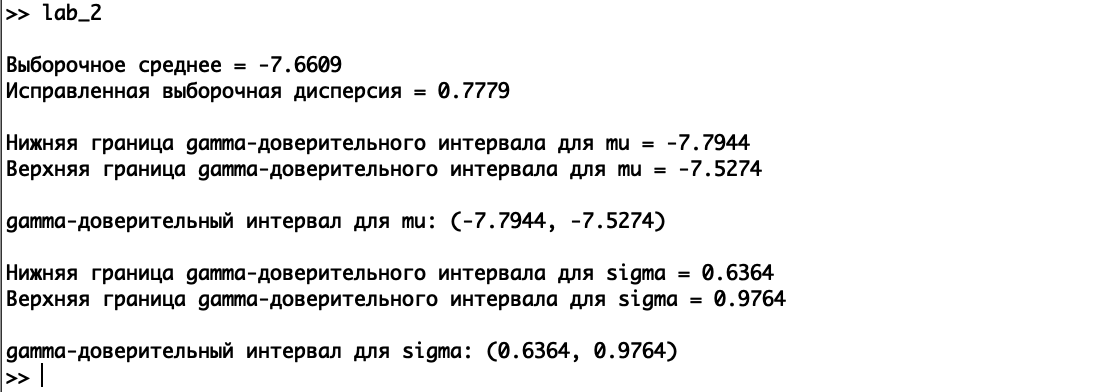
\includegraphics[scale=1]{img/result.png}
	\caption{Результаты расчетов для выборки из индивидуального варианта}   
	\label{fig:result}
\end{figure}

\begin{figure}[h]
	\centering
	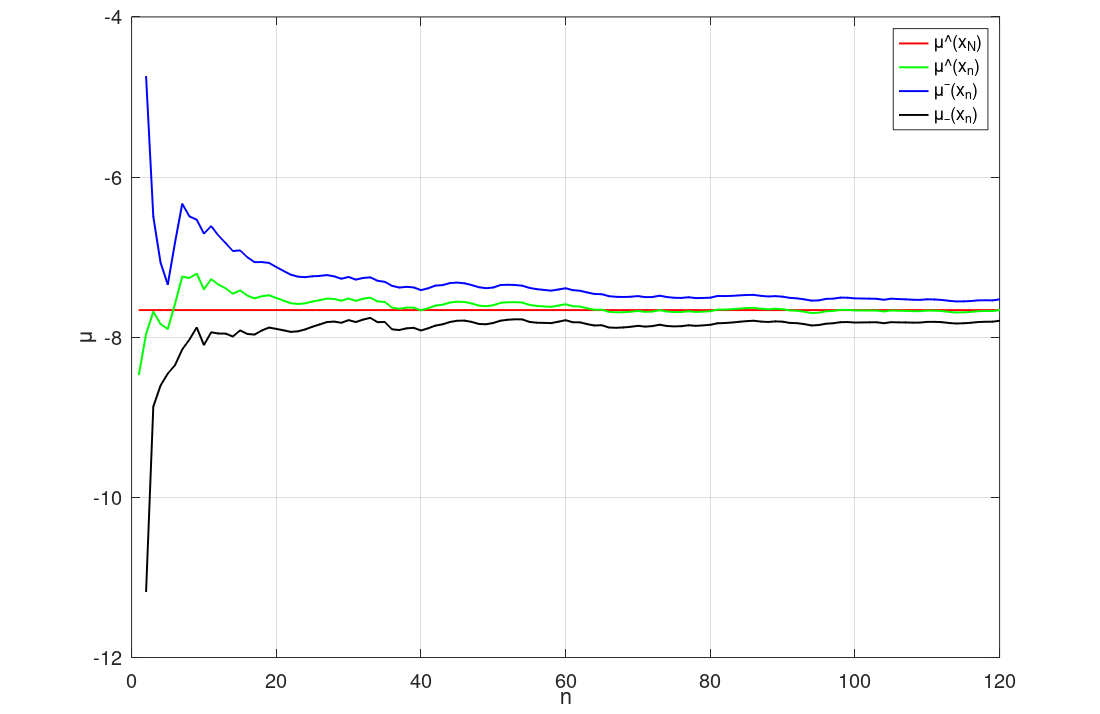
\includegraphics[scale=0.9]{img/mu.png}
	\caption{График для математического ожидания}
	\label{fig:mu}
\end{figure}

\begin{figure}[h]
	\centering
	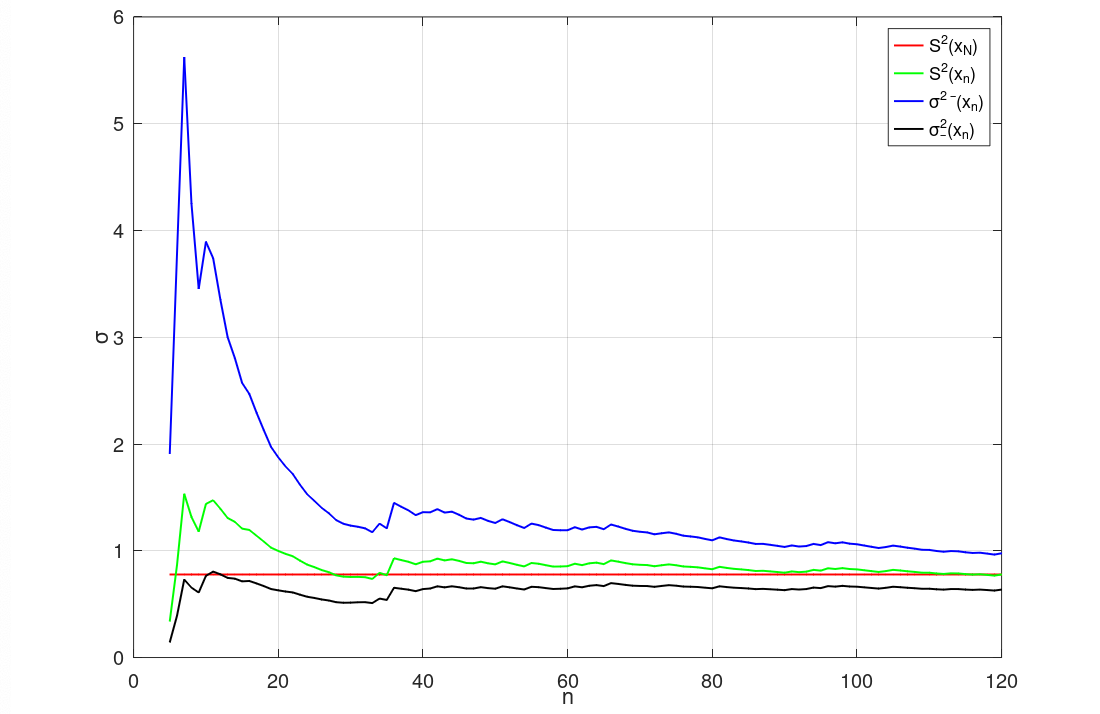
\includegraphics[scale=0.9]{img/sigma.png}
	\caption{График для дисперсии}
	\label{fig:sigma}
\end{figure}

\end{document}
